\begin{figure*}[t]
	\centering
	\addtolength{\tabcolsep}{-4.5pt}
	\begin{tabular}{ccccccccc}
		Photo & Sample-1 & Sample-2 & Sample-3 & & Photo & Sample-1 & Sample-2 & Sample-3
		\\
		\begin{overpic}[width=\resultwidth]{real/bump_1/target.jpg}
			\imglabel{Bump-3}
		\end{overpic} &
		\includegraphics[width=\resultwidth]{real/bump_1/good1.jpg} &
		\includegraphics[width=\resultwidth]{real/bump_1/good2.jpg} &
		\includegraphics[width=\resultwidth]{real/bump_1/bad1.jpg} &
		&
		\begin{overpic}[width=\resultwidth]{real/bump_2/target.jpg}
			\imglabel{Bump-4}
		\end{overpic} &
		\includegraphics[width=\resultwidth]{real/bump_2/good1.jpg} &
		\includegraphics[width=\resultwidth]{real/bump_2/good2.jpg} &
		\includegraphics[width=\resultwidth]{real/bump_2/bad1.jpg}
		\\
		\begin{overpic}[width=\resultwidth]{real/leather_1/target.jpg}
			\imglabel{Leather-3}
		\end{overpic} &
		\includegraphics[width=\resultwidth]{real/leather_1/good1.jpg} &
		\includegraphics[width=\resultwidth]{real/leather_1/good2.jpg} &
		\includegraphics[width=\resultwidth]{real/leather_1/bad1.jpg} &
		&
		\begin{overpic}[width=\resultwidth]{real/leather_2/target.jpg}
			\imglabel{Leather-4}
		\end{overpic} &
		\includegraphics[width=\resultwidth]{real/leather_2/good1.jpg} &
		\includegraphics[width=\resultwidth]{real/leather_2/good2.jpg} &
		\includegraphics[width=\resultwidth]{real/leather_2/bad1.jpg}
		\\
		\begin{overpic}[width=\resultwidth]{real/leather_3/target.jpg}
			\imglabel{Leather-5}
		\end{overpic} &
		\includegraphics[width=\resultwidth]{real/leather_3/good1.jpg} &
		\includegraphics[width=\resultwidth]{real/leather_3/good2.jpg} &
		\includegraphics[width=\resultwidth]{real/leather_3/bad1.jpg} &
		&
		\begin{overpic}[width=\resultwidth]{real/leather_4/target.jpg}
			\imglabel{Leather-6}
		\end{overpic} &
		\includegraphics[width=\resultwidth]{real/leather_4/good1.jpg} &
		\includegraphics[width=\resultwidth]{real/leather_4/good2.jpg} &
		\includegraphics[width=\resultwidth]{real/leather_4/bad1.jpg}
		\\
		\begin{overpic}[width=\resultwidth]{real/plaster_1/target.jpg}
			\imglabel{Plaster-3}
		\end{overpic} &
		\includegraphics[width=\resultwidth]{real/plaster_1/good1.jpg} &
		\includegraphics[width=\resultwidth]{real/plaster_1/good2.jpg} &
		\includegraphics[width=\resultwidth]{real/plaster_1/bad1.jpg} &
		&
		\begin{overpic}[width=\resultwidth]{real/plaster_2/target.jpg}
			\imglabel{Plaster-4}
		\end{overpic} &
		\includegraphics[width=\resultwidth]{real/plaster_2/good1.jpg} &
		\includegraphics[width=\resultwidth]{real/plaster_2/good2.jpg} &
		\includegraphics[width=\resultwidth]{real/plaster_2/bad1.jpg}
		\\
		\begin{overpic}[width=\resultwidth]{real/flake_1/target.jpg}
			\imglabel{Metallicflake-3}
		\end{overpic} &
		\includegraphics[width=\resultwidth]{real/flake_1/good1.jpg} &
		\includegraphics[width=\resultwidth]{real/flake_1/good2.jpg} &
		\includegraphics[width=\resultwidth]{real/flake_1/bad1.jpg} &
		&
		\begin{overpic}[width=\resultwidth]{real/flake_2/target.jpg}
			\imglabel{Metallicflake-4}
		\end{overpic} &
		\includegraphics[width=\resultwidth]{real/flake_2/good1.jpg} &
		\includegraphics[width=\resultwidth]{real/flake_2/good2.jpg} &
		\includegraphics[width=\resultwidth]{real/flake_2/bad1.jpg}
		\\
		\begin{overpic}[width=\resultwidth]{real/metal_1/target.jpg}
			\imglabel{Brushmetal-3}
		\end{overpic} &
		\includegraphics[width=\resultwidth]{real/metal_1/good1.jpg} &
		\includegraphics[width=\resultwidth]{real/metal_1/good2.jpg} &
		\includegraphics[width=\resultwidth]{real/metal_1/bad1.jpg} &
		&
		\begin{overpic}[width=\resultwidth]{real/wood_1/target.jpg}
			\imglabel{Wood-3}
		\end{overpic} &
		\includegraphics[width=\resultwidth]{real/wood_1/good1.jpg} &
		\includegraphics[width=\resultwidth]{real/wood_1/good2.jpg} &
		\includegraphics[width=\resultwidth]{real/wood_1/bad1.jpg}
		\\
		\begin{overpic}[width=\resultwidth]{real/wood_2/target.jpg}
			\imglabel{Wood-4}
		\end{overpic} &
		\includegraphics[width=\resultwidth]{real/wood_2/good1.jpg} &
		\includegraphics[width=\resultwidth]{real/wood_2/good2.jpg} &
		\includegraphics[width=\resultwidth]{real/wood_2/bad1.jpg} &
		&
		\begin{overpic}[width=\resultwidth]{real/wood_3/target.jpg}
			\imglabel{Wood-5}
		\end{overpic} &
		\includegraphics[width=\resultwidth]{real/wood_3/good1.jpg} &
		\includegraphics[width=\resultwidth]{real/wood_3/good2.jpg} &
		\includegraphics[width=\resultwidth]{real/wood_3/bad1.jpg}
	\end{tabular}
	\captionsetup{labelfont=bf,textfont=it}
	\caption{\label{fig:real}
		\textbf{Results} of our MCMC sampling on \textbf{real} inputs. For each example, the first column is the real target image (photo). We show MCMC samples in the other columns, where sample-1 and sample-2 are chosen closer to the peak of the posterior distribution, and sample-3 is further away. Note that the target images for Plaster-4 and Wood-5 are captured under natural illumination, while the corresponding synthetic images still assume collocated flash illumination; despite this mismatch, the estimated material parameters are still reasonable. Note, target images for Leather-4, Leather-6 and Wood-4 are from the publicly released dataset of \cite{Aittala2016}. For more results please refer to supplemental materials.
	}
\end{figure*}
